% Chapter 1

\chapter{Introducción general} % Main chapter title

\label{Chapter1} % For referencing the chapter elsewhere, use \ref{Chapter1} 

En este capítulo se describe el contexto actual del cual parte el trabajo y el estado del arte de los sistemas de llamado a enfermera. Además se presentan los objetivos, el alcance del trabajo y se expone su justificación.

\label{IntroGeneral}

%----------------------------------------------------------------------------------------

% Define some commands to keep the formatting separated from the content 
\newcommand{\keyword}[1]{\textbf{#1}}
\newcommand{\tabhead}[1]{\textbf{#1}}
\newcommand{\code}[1]{\texttt{#1}}
\newcommand{\file}[1]{\texttt{\bfseries#1}}
\newcommand{\option}[1]{\texttt{\itshape#1}}
\newcommand{\grados}{$^{\circ}$}

%----------------------------------------------------------------------------------------

%\section{Introducción}

%----------------------------------------------------------------------------------------
\section{Antecedentes y análisis de contexto}
\label{sec:AntyCont}

SURIX es una empresa argentina fundada en 1998, que se dedica al desarrollo de sistemas de control de acceso basados en tecnología IP. Actualmente ofrece líneas de productos para el hogar y edificios, aplicaciones tecnológicas personalizadas para corporaciones, industrias, hospitales, centros comerciales, autopistas y entes gubernamentales. Estos productos se exportan a más de 14 países para diversas aplicaciones, por lo que tiene oficinas en Israel y México \cite{surix}.

Entre los productos ofertados por SURIX, se destaca el sistema de llamado a enfermera. Este consta de un dispositivo llamador, que se conecta por cable a un terminal de sala, que a su vez se conecta a través de una red con el terminal de enfermería \cite{helpip}.

Desde el dispositivo llamador, el paciente puede encender la luz de lectura o –lo que es más relevante– requerir la atención del personal de servicio a la habitación. En caso de necesitar atención, el terminal de sala iniciará una llamada VoIP con el terminal de enfermería.

El sistema diferencia un llamado para servicio a la habitacion, asistencia en el baño o asistencia en caso de paro cardíaco, y si fue atendido por enfermería remotamente o se está en presencia de la enfermera. También indica cuando concluye el servicio de la enfermera en el cuarto.

Además permite visibilizar la solicitud y tipo de solicitud, por medio de una luminaria ubicada en el pasillo sobre la puerta de la habitación , que se puede configurar para iluminarse de diversos colores o encenderse intermitentemente en función del tipo de solicitud del paciente.

En la terminal de enfermería se dispone de un panel donde se puede visualizar el estado de cada cama, y el terminal de sala actualmente sólo puede conectarse a dos dispositivos llamadores.

En el mercado existen varias soluciones similares a la que se desea desarrollar, entre las que podemos mencionar:

\begin{itemize}
\item MMCALL: sistema que utiliza tecnologías inalámbricas y dispone de pulsadores de llamada colocados en las habitaciones y baños de los pacientes, a través de los cuales solicitan asistencia presionando un botón. La estación de enfermería muestra el número de habitación o cama asignado a ese pulsador de llamada y simultáneamente activa un cronómetro para garantizar una atención oportuna, de manera que si la llamada no es respondida envía un recordatorio tanto a la estación de enfermería como a todos los relojes inalámbricos, con los que cada miembro del personal puede ser equipado, para asegurar que la llamada sea respondida sin importar en qué parte del hospital se encuentren. Todas las llamadas se registran en la estación de enfermería, lo cual permite sacar reportes de desempeño y rendimiento. El alcance de la señal es de 70 a 80 metros, pero se puede extender utilizando amplificadores y repetidores de señal \cite{mmcall}.	

\item Helpnex: sistema modular que utiliza tecnología IP, dispone de pulsadores para cama y baño que permiten que el paciente solicite asistencia presionando un botón, y permite visualizar y atender el requerimiento, pudiendo detallar el motivo o añadir todo tipo de observaciones sobre la solicitud. Todas las alarmas y tareas quedan registradas en una base de datos. Ofrece control sobre personas en general, pudiendo obtener su ubicación en tiempo real, mediante un tag pequeño y compacto, que permite la localización de la persona, a través de radiofrecuencia sobre las principales salidas del centro, con distinción entre cercanía o apertura de una puerta, con visualización de alarmas en el plano en tiempo real. Permite también alarma para pasillo con diferentes códigos de colores, emitiendo indicación sonora y luminosa. Además ofrece la posibilidad de disponer de un puesto de control para la emisión de informes personalizados, permitiendo conocer todo lo ocurrido en el centro de atención medica. \cite{helpnex}.

\item Llamador de enfermería inalámbrico SEI: sistema desarrollado para clínicas, hospitales, geriátricos, hogares de ancianos o casas particulares con personas con movilidad reducida. Dispone de un llamador en cada habitación identificado por un número, cada uno de estos llamadores dispone de tantos pulsadores como camas posea la habitación. Cuando el paciente presiona el pulsador, se reporta inalámbricamente a una central receptora, encendiendo el LED correspondiente a dicha habitación, y una señal sonora advierte del llamado. Mientras existan llamados activos se oirá un “bip” cada 10 segundos alertando a la persona a cargo del llamado pendiente. Si el llamado lleva activo un tiempo mayor a 5 minutos el LED comenzará a parpadear alertando la demora. Para cancelar el llamado la enfermera o persona a cargo debe dirigirse a la habitación correspondiente y presionar el botón “cancelar” del llamador. Mientras el llamado esté activo, en el llamador destellará un LED indicando dicho estado. El alcance de la señal inalámbrica es de 30 a 35 metros que puede extenderse mediante el uso de retransmisores \cite{sei}.

\end{itemize}

En la tabla \ref{tab:sistemasDeLLamadoEnfermera} se resumen las características del sistema de llamado a enfermera de SURIX y de los demás sistemas mencionados.

\begin{table}[h]
	\centering
	\caption[Sistemas de llamado a enfermera]{Tabla comparativa de los sistemas de llamado a enfermera disponibles en el mercado}
	\begin{tabular}{l c c c c}    
		\toprule
		\textbf{Característica} 	 & \textbf{SURIX} & \textbf{MMCALL} & \textbf{Helpnex} & \textbf{SEI}\\
		\midrule
		Dispositivo llamador inalámbrico                                                    &   &   &   & X \\
Central de enfermera inalámbrica                                                    &   & X & X & X \\
\begin{tabular}[c]{@{}l@{}}Aviso de presencia de \\ enfermera por RFID\end{tabular} & X &   & X &   \\
Sistema de localización de pacientes                                                &   &   & X &   \\
Panel de control                                                                    & X & X & X & X \\
Alarma de pasillo configurable                                                      & X & X & X &   \\
Emisión de informes                                                                 & X & X & X &   \\
		\bottomrule
		\hline
	\end{tabular}
	\label{tab:sistemasDeLLamadoEnfermera}
\end{table}

En la figura \ref{fig:sistemasDeLLamadoactuales} se ilustran los distintos equipos llamadores que se han presentado en esta sección.

\begin{figure}[!h]
	\centering
   	\begin{subfigure}[b]{0.5\textwidth}
   		\centering
      	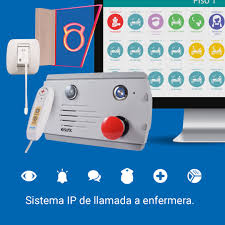
\includegraphics[width=0.6\textwidth]{helpIp.jpeg}
      	\caption{Help IP SURIX.}
   	\end{subfigure}%
   	\begin{subfigure}[b]{0.5\textwidth}
   		\centering
      	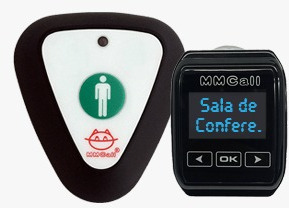
\includegraphics[width=0.7\textwidth]{mmcall.jpeg}
      	\caption{MMCALL.}
   	\end{subfigure}%
   	\newline
   	\begin{subfigure}[b]{0.5\textwidth}
   		\centering
      	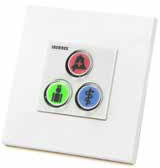
\includegraphics[width=0.6\textwidth]{helpnex.jpeg}
      	\caption{Helpnex.}
   	\end{subfigure}%
   	\begin{subfigure}[b]{0.5\textwidth}
   		\centering
      	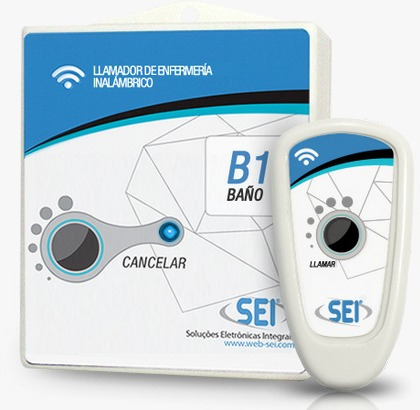
\includegraphics[width=0.7\textwidth]{sei.jpeg}
      	\caption{Llamador de enfermería inalámbrico SEI.}
   	\end{subfigure}%
	\caption{Llamadores de enfermera disponibles en el mercado.}
	\label{fig:sistemasDeLLamadoactuales}
\end{figure}


%----------------------------------------------------------------------------------------

\section{Objetivos y Alcance}

\subsection{Objetivos}

El objetivo general de este trabajo es dotar de conectividad Bluetooth al sistema actual de llamado a enfermera de SURIX. Esto permitirá que el sistema de SURIX cuente con un dispositivo llamador inalámbrico, y una central de enfermera inalámbrica. Adicionalmente permitirá en un futuro que se implemente un sistema de localización de pacientes.

Para el logro del objetivo planteado el trabajo contempla:

\begin{itemize}

\item El diseño e implementación de un módulo de expansión que permita dotar de conectividad Bluetooth a la terminal de sala del sistema actual de SURIX.

\item El diseño e implementación de un nuevo dispositivo llamador con conectividad Bluetooth.

\item El desarrollo del firmware para el módulo de expansión diseñado.

\item El desarrollo del firmware para el nuevo dispositivo llamador.

\item El desarrollo del firmware de la terminal de sala para el control de módulo de expansión diseñado.

\end{itemize}

\subsection{Alcance}

El alcance del trabajo está definido por las siguientes consideraciones:

\begin{itemize}
\item Si bien en el trabajo uno de los objetivos es desarrollar el firmware para control del módulo de expansión, esto no implica sustituir el firmware de la terminal de sala por uno nuevo, sino sólo escribir el módulo que permita interactuar a la terminal de sala con el módulo de expansión diseñado, ya que el resto del sistema actual se seguirá utilizando.	

\item Debido a que el diseño del dispositivo llamador debe ser de bajo consumo de energía, este no dispondrá de un parlante, por lo que no se considera el desarrollo de firmware que envíe audio al dispositivo llamador, y la salida de audio se mantendrá en la terminal de sala, como ocurre con el sistema actual.

\item Aunque el diseño del dispositivo llamador implica elegir una fuente de alimentación, el trabajo no contempla diseñar un sistema de recarga para la batería.

\end{itemize}

%----------------------------------------------------------------------------------------

\section{Justificación}

El trabajo permite ampliar la capacidad de conexión de la terminal de sala, que actualmente está limitada a sólo dos dispositivos llamadores, de manera que será posible conectar un mayor número de dispositivos llamadores.

Adicionalmente, como los equipos se conectan mediante cables puede ocurrir que queden fuera de servicio por rotura de los mismo. Este problema se vería resuelto al dotar de conectividad Bluetooth al dispositivo.

Quitar el cable también posibilita que los pacientes que por su estado se encuentren débiles puedan acercar el llamador a su boca haciendo que sea más fácil escuchar su voz.

El hecho de que el dispositivo llamador sea inalámbrico permite que pueda ser utilizado en distintos lugares, lo que permite reorganizar fácilmente una sala, o incluso usar el dispositivo llamador en otra sala, donde sea requerido.

Por otro lado, el dotar de conectividad Bluetooth al sistema actual permitirá a SURIX posicionar este producto para competir con otros sistemas existentes en el mercado, que ya ofrecen esta característica.
